\documentclass[letterpaper,12pt]{article}

% Encoding
\usepackage[utf8]{inputenc}

% Page structure
\usepackage{geometry}
\geometry{margin=2.54cm}
\geometry{top=1.54cm}

% Titles
\usepackage{sectsty}
\allsectionsfont{\sffamily\mdseries\upshape}

% Headers and Footers
\usepackage{fancyhdr}
\pagestyle{fancy}

% Graphics, figures and plots
\usepackage{graphicx}
\usepackage{float}
\usepackage{pgfplots}
\usepackage{caption}
\usepackage{subcaption}

% Etc
\usepackage{hyperref}

% Bibliography
\usepackage[numbers]{natbib}

%%%%%%%%%%
% Math
\usepackage{amsmath}
\usepackage{amsthm}
\usepackage{amsfonts}
\usepackage{amssymb}
\usepackage{amscd}
\usepackage{eurosym}
\usepackage{mathrsfs}
\usepackage{mathtools}
\usepackage{bm} % defines a com­mand \bm which makes its ar­gu­ment bold
\usepackage{bbm}

%%%% Mathematical Environments
\theoremstyle{plain}
\newtheorem{theorem}{Theorem}[section]
\newtheorem{lemma}[theorem]{Lemma}
\newtheorem{corollary}[theorem]{Corollary}
\newtheorem{proposition}[theorem]{Proposition}
\newtheorem{conjecture}[theorem]{Conjecture}

\theoremstyle{definition}
\newtheorem{definition}[theorem]{Definition}
\newtheorem{example}[theorem]{Example}

\theoremstyle{remark}
\newtheorem{remark}[theorem]{Remark}
\newtheorem{note}[theorem]{Note}
\newtheorem{case}[theorem]{Case}

%%%%%%%%%%
% Pseudocode
\usepackage{algorithm}
\usepackage{algpseudocode}

%%%%%%%%%%
% Operators
\DeclareMathOperator*{\argmax}{arg\,max}
\DeclareMathOperator*{\argmin}{arg\,min}
\DeclareMathOperator*{\Exp}{\mathbb{E}}
\DeclareMathOperator*{\Var}{\text{Var}}
\DeclareMathOperator*{\Cov}{\text{Cov}}

%%%%%%%%%%
% Paired -- \command* will automatically resize
\DeclarePairedDelimiter\paren{(}{)}           % (parentheses)
\DeclarePairedDelimiter\ang{\langle}{\rangle} % <angle brackets>
\DeclarePairedDelimiter\abs{\lvert}{\rvert}   % |absolute value|
\DeclarePairedDelimiter\norm{\lVert}{\rVert}  % ||norm||
\DeclarePairedDelimiter\bkt{[}{]}             % [brackets]
\DeclarePairedDelimiter\set{\{}{\}}           % {braces}

%%%%%%%%%%
% Macros
% Bidders
\newcommand{\bidders}[1][]{N}
\newcommand{\numbidders}[1][]{n}
% Goods
\newcommand{\goods}[1][]{G}
\newcommand{\numgoods}[1][]{g}
% Allocations
\newcommand{\alloc}[1][]{x_{#1}}
\newcommand{\allocvec}[1][]{\mathbf{\alloc}}
\newcommand{\intalloc}[1][]{{\hat{\alloc}}_{#1}}
\newcommand{\intallocvec}[1][]{\mathbf{\intalloc}}
% Valuations
\newcommand{\val}[1][]{v_{#1}}
\newcommand{\valvec}[1][]{\mathbf{\val}_{#1}}
\newcommand{\valz}[1][]{z_{#1}}
\newcommand{\valzvec}[1][]{\mathbf{\valz}_{#1}}
\newcommand{\valspace}[1][]{T_{#1}}
\newcommand{\valspacesize}[1][]{M_{#1}}
% Payment
\newcommand{\payment}[1][]{p_{#1}}
\newcommand{\paymentvec}[1][]{\mathbf{\payment}_{#1}}
% Virtual values (continuous and discrete)
\newcommand{\virval}[1][]{\varphi_{#1}}
\newcommand{\virvalvec}[1][]{\mathbf{\virval}_{#1}}
\newcommand{\virvald}[1][]{\psi_{#1}}
\newcommand{\virvaldvec}[1][]{\mathbf{\virvald}_{#1}}

%%%%%%%%%%

\title{Unit demand experiments}

\author{Enrique Areyan Viqueira and Amy Greenwald}


%%%%

\begin{document}

\maketitle

\section{Introduction}

This document summarizes experiments we performed in the case of a centralized combinatorial matching markets
where bidders have unit demand valuations.

\section{Experimental setup}

Each point $(r,s)$ in the graphs below represents the seller revenue $s$ as a function of reserve price $r$ in a market with $n$ items and $m$ bidders, 
where each bidder has unit demand valuation on the items. (The values of $n$ and $m$ are in the title of each graph). 
Note that a market where there are $n$ items and $m$ bidders, each of which has unit demand valuation, is completely specified 
by a $n$ by $m$ valuation matrix $V$, where entry $V_{ij}$ represents the valuation bidder $j$ has for item $i$. 

Each point $(r,s)$ is the average over 1000 independently drawn random valuation matrices, where each entry $V_{ij}$ is drawn from a continuous uniform distribution 
with support [1,10]. We also control for the connectivity of the market with a parameter $p$ that specifies, for each valuation $V_{ij}$, the probability that it is
drawn from a [1,10] uniform distribution or is $-\infty$.
To obtain a seller revenue from a random matrix $V$ and reserve price $r$, we do the following:
\begin{enumerate}
 \item ``Shift'' matrix $V_{ij}$ by $r$. This operation consists of discounting the valuation of each bidder for each item according to reserve price $r$. 
	Concretely, from $V$ we construct a valuation matrix that respects reserve price $r$, call it $V^r$, by setting $V^r_{ij} = V_{ij} - r$ if $V_{ij} - r>0$
	and -$\infty$ otherwise. Thus, if an item becomes too expensive for a bidder at reserve price $r$, the bidder no longer has a valuation for it.
 \item Run MaxWEQ on $V^r$ to obtain a maximum Walrasian Equilibrium, i.e., an allocation $X^r$ and prices $P^r$, such that unallocated items are prices at zero 
	and bidders are envy-free.
 \item Obtain prices for the original market $V$ by adding the reserve to all prices in $P^r$. Concretely, define price vector $P$ by letting $P_i = P^r_i + r$ for every item $i$.
 \item Finally, compute the seller revenue from allocation $X^r$ using prices $P$. In other words, the seller revenue is defined to be the sum of the prices (plus reserve) of allocated items.
\end{enumerate}
This procedure produces a Walrasian Equilibrium with reserve price $r$.
\section{Graphs}
Over-supplied markets: Supply $>$ demand (more items than bidders)

\hspace*{-0.75in}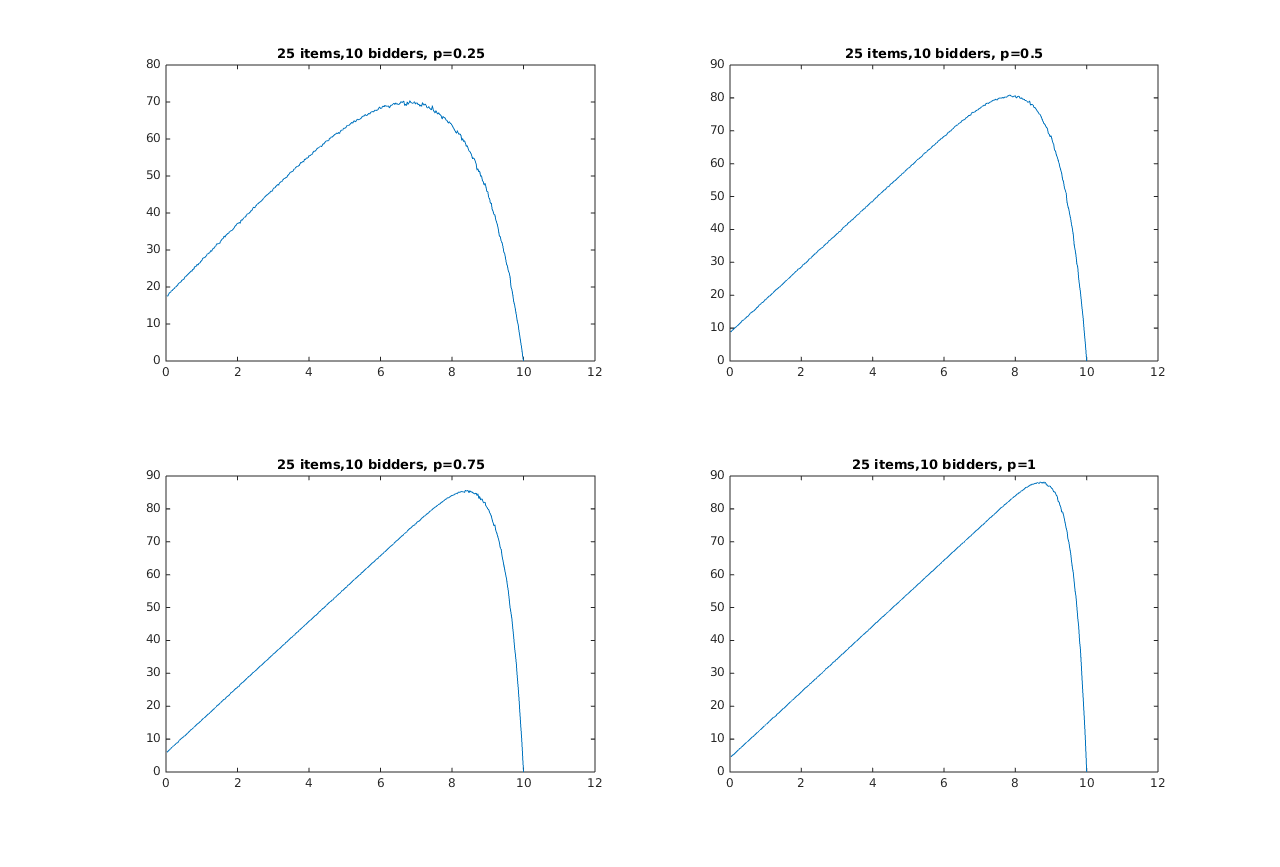
\includegraphics[width=38em]{../unit-demand/unitdemand-25-10.png}

Equally supplied markets: Supply $=$ demand (same number of items than bidders)

\hspace*{-0.75in}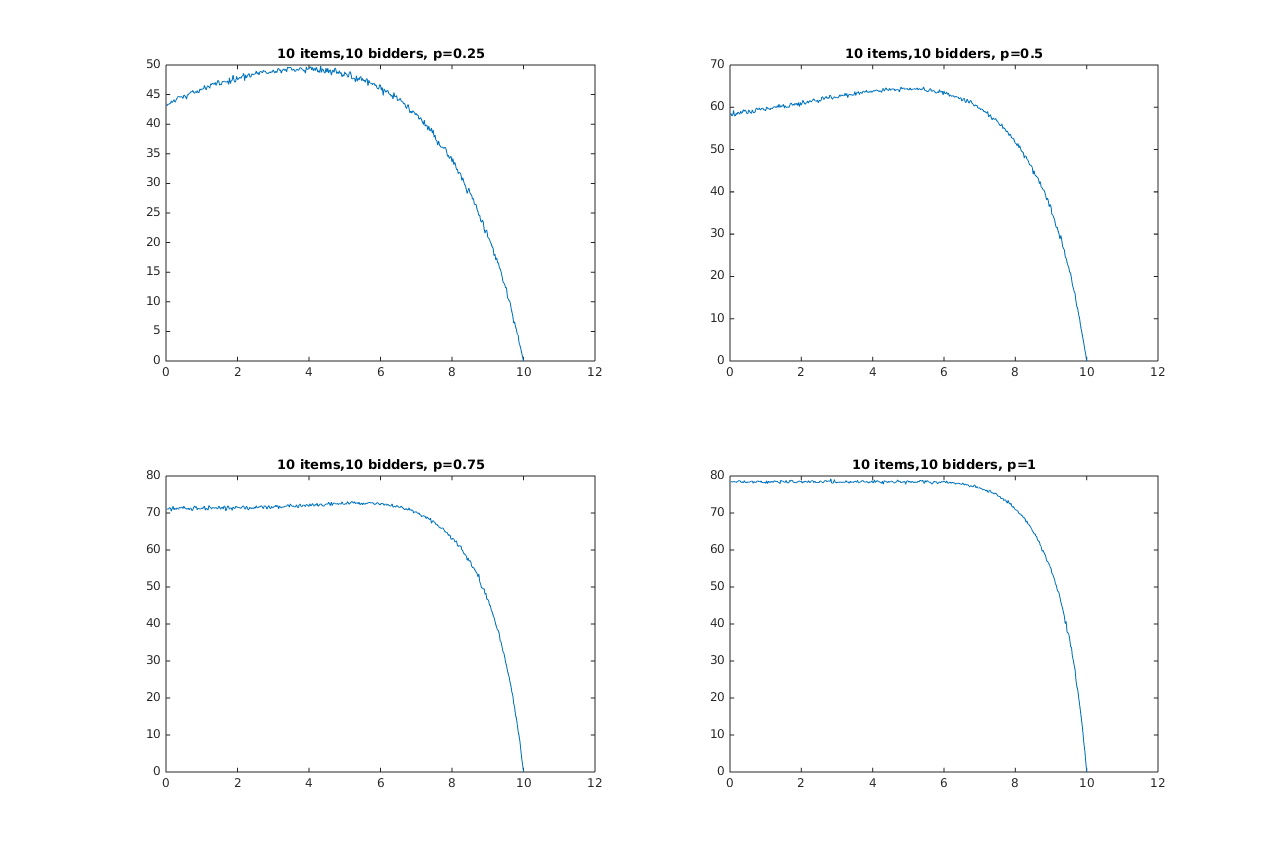
\includegraphics[width=38em]{../unit-demand/unitdemand-10-10.png}

Under-supplied markets: Supply $<$ demand (more bidders than items)

\hspace*{-0.75in}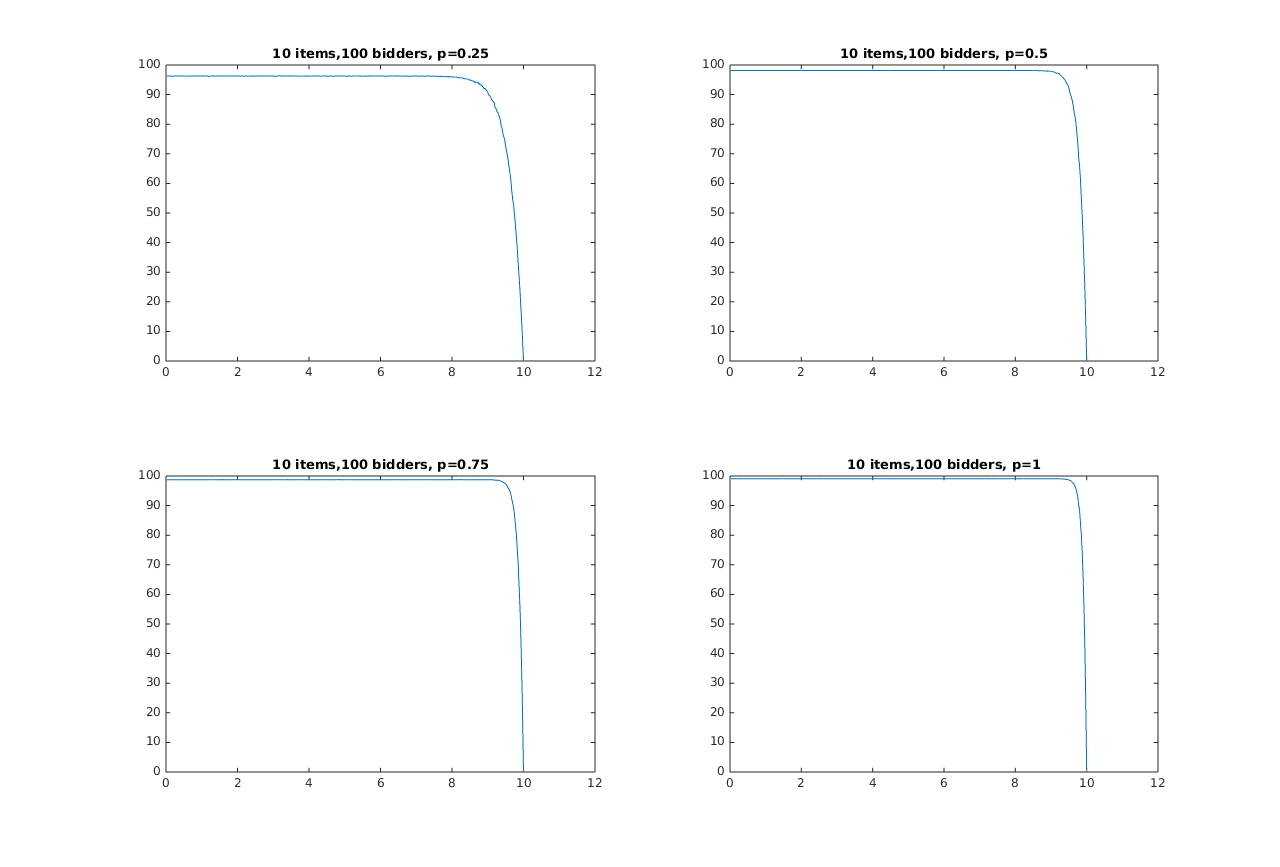
\includegraphics[width=38em]{../unit-demand/unitdemand-10-100.png}

\section{Preliminary Analysis}

First, note that, since rewards are constraint to lie between [1,10], any market with a reserve price $r$ greater than 10 will have 0 revenue, since 
no bidder can afford any item. 

Also, note that, for markets with full valuation $p=1$, if the number of items is greater than the number of bidders then not all items will be allocated.
Since unallocated items will be priced at exactly the reserve (market clearance condition) and bidders are envy-free, revenue for this markets is sensitive to reserve prices. 
This explains why in the first set of graphs (markets with 25 items and  10 bidders), revenue is low for low reserve prices and increases almost linearly 
before dropping at reserve prices close to 10. 

In markets where supply = demands or supply $<$ demand, all items will be allocated and thus, we get the market clearance condition for free.
In this case the structure of our experiments is such that using a reserve price makes virtually no difference (in expectation).
Consider the case $p=1$. Since all bidders have valuations for all items and we have at least 10 bidders, we expect to have each bidder valuating 
at least (roughly) one item close to 10. These are the items that get allocated and thus, we get almost all the possible revenue from these markets
at any reserve price less than 10 (in reality reserve less than 8.5 approximately).

%%%%%%%%%%
% References and End of Paper
%\bibliographystyle{plainnat}
%\bibliography{bibliography}

\end{document}